\chapter{Finite automata minimization algorithms}

\section{Introduction}

\section{Brzozowski's algorithm}

\begin{flushleft}
$\epsilon-free$ FA: $M_0=(Q_0,V,T_0,\emptyset,S_0,F_0)$ \\
to be minimized $DFA$: $M_2=(Q_2,V,T_2,\emptyset,S_2,F_2)$ \\
intermediate $NFA$: $M_1=(Q_1,V,T_1,\emptyset,S_1,F_1)$\\
\end{flushleft}

NFA: $M_1 \to $ DFA: $M_2, M_2=suseful_s\circ subsetopt(M_1)$
\begin{align*}
& q_0,q_1\in Q_1,Q_2\subseteq\mathbb{P}(Q_1),\forall p\in  Q_2,p=(q_0,q_1)\\
& \overrightarrow{L}_{M_2}(p)=\overrightarrow{L}_{M_1}(q_0)\cup  \overrightarrow{L}_{M_1}(q_1)\\
& \Rightarrow \\
& \overrightarrow{L}_{M_2}(p)=\bigcup_{q\in p}\overrightarrow{L}_{M_1}(q)\\
& \Rightarrow 
\end{align*}

\begin{figure}[htbp]
	\begin{tikzpicture}
	\matrix (a) [matrix of math nodes,row sep=3em,
	column sep=5em, nodes in empty cells]
	{ Q_1 &  P(Q_1) \\ 
		&  D(Q_2) \\};
	\path[>=latex,->] 
	(a-1-1) edge node [auto] {$subsetopt$} (a-1-2)
	edge node [auto,swap] {$$} (a-2-2)
	(a-1-2) edge node [auto] {$useful_s$} (a-2-2)
	;
	\end{tikzpicture}
	\caption{$M_2=suseful_s\circ subsetopt(M_1)$}
\end{figure}

\begin{figure}[htbp]
	\subfigure[$M_1=(Q_1,V,T_1,\emptyset,S_1,F_1)$] { \label{fig:a} 
	\begin{tikzpicture}[->,>=stealth',shorten >=1pt,auto,node distance=2cm, semithick]
		\tikzstyle{every state}=[minimum size=0.1mm]
		\node[state] (q)  [] {$q$};
		\node[state] (q0) [above right of=q] {$q_0$};
		\node[state] (q1) [below right of=q] {$q_1$};
		\node[state] (f1)  [below right of=q0] {$f_1$};
		\path 
		(q) edge [] node {$a$} (q0)
		    edge [swap] node {$a$} (q1)
		(q0) edge [] node {$\overrightarrow{L}_{M_1}(q_0)$} (f1)
		(q1) edge [swap] node {$\overrightarrow{L}_{M_1}(q_1)$} (f1)
		;
	\end{tikzpicture}
    }
    \hspace{2cm}
	\subfigure[$M_2=(Q_2,V,T_2,\emptyset,S_2,F_2)$] { \label{fig:b}
    \begin{tikzpicture}[->,>=stealth',shorten >=1pt,auto,node distance=3cm, semithick,scale=4]
    	\tikzstyle{every state}=[minimum size=0.1mm]
    	\node[state] (q01)  {$(q_0,q_1)$};
    	\node[state] (f2)  [right of=q01] {$f_2$};
    	\path 
    	(q01) edge [bend left] node {$\overrightarrow{L}_{M_1}(q_0)$} (f2)
    	(q01) edge [bend right,swap] node {$\overrightarrow{L}_{M_1}(q_1)$} (f2)
    	;
    \end{tikzpicture}
    }
	\caption{$M_2=suseful_s\circ subsetopt(M_1)$}
\end{figure}

\begin{figure}[htbp]
	\subfigure[$M_0=(Q_0,V,T_0,\emptyset,S_0,F_0)$] {
		\begin{tikzpicture}[->,>=stealth',shorten >=1pt,auto,node distance=2cm, semithick]
		\tikzstyle{every state}=[minimum size=0.1mm]
		\node[state,accepting] (q2) []{$q_2$};
		\node[state,initial] (q0) [above left of=q2] {$q_0$};
		\node[state] (q1) [above right of=q2] {$q_1$};
		\path
		(q0) edge[bend left] node {$0$} (q1)
		(q1) edge[bend left] node {$0$} (q0)
		(q0) edge[swap] node {$1$} (q2)
		(q1) edge[] node {$1$} (q2)
		(q2) edge[loop below] node {$0,1$} (q2)
		;
		\end{tikzpicture}
	}
    \hspace{1cm}
	\subfigure[$M^R_0=(Q_0,V,T_0,\emptyset,S_0,F_0)^R=(Q_0,V,T^R,\emptyset,F_0,S_0)$]{
		\begin{tikzpicture}[->,>=stealth',shorten >=1pt,auto,node distance=2cm, semithick]
		\tikzstyle{every state}=[minimum size=0.1mm]
		\node[state,initial] (q2) []{$q_2$};
		\node[state,accepting] (q0) [above left of=q2] {$q_0$};
		\node[state] (q1) [above right of=q2] {$q_1$};
		\path
		(q1) edge[bend right,swap] node {$0$} (q0)
		(q0) edge[bend right,swap] node {$0$} (q1)
		(q2) edge[] node {$1$} (q0)
		(q2) edge[swap] node {$1$} (q1)
		(q2) edge[loop below] node {$0,1$} (q2)
		;
		\end{tikzpicture}
	}
    \newline
	\subfigure[$useful_s\circ subsetopt\circ R(M_0)$]{
		\begin{tikzpicture}[->,>=stealth',shorten >=1pt,auto,node distance=2cm, semithick]
		\tikzstyle{every state}=[minimum size=0.1mm]
		\node[state,initial] (q2) []{$q_2$};
		\node[state,accepting] (q0) [above of=q2] {$\{q_0,q_1,q_2\}$};
		\path
		(q2) edge[] node {$1$} (q0)
		(q0) edge[loop above] node {$0,1$} (q0)
		(q2) edge[loop below] node {$0$} (q2)
		;
	\end{tikzpicture}
	}
    \hspace{3cm}
    \subfigure[$M_1=R\circ useful_s\circ subsetopt\circ R(M_0)$]{
    	\begin{tikzpicture}[->,>=stealth',shorten >=1pt,auto,node distance=2cm, semithick]
    	\tikzstyle{every state}=[minimum size=0.1mm]
    	\node[state,accepting] (q2) []{$q_2$};
    	\node[state,initial] (q0) [above of=q2] {$\{q_0,q_1,q_2\}$};
    	\path
    	(q0) edge[] node {$1$} (q2)
    	(q0) edge[loop above] node {$0,1$} (q0)
    	(q2) edge[loop below] node {$0$} (q2)
    	;
    	\end{tikzpicture}
    }
    \caption{$M_1=R\circ useful_s\circ subsetopt\circ R(M_0)$}
\end{figure}

\begin{figure}[htbp]
	\begin{align*}
	\text{start: } &U=\{q_2\}\\
	u=q_2: & T(q_2,0)=\{q_2\},T(q_2,1)=\{q_0,q_1,q_2\} \\
	&\text{add new start to $D$, } D=\{q_2,\{q_0,q_1,q_2\}\} \\
	u=\{q_0,q_1,q_2\}:& T(\{q_0,q_1,q_2\},0)=T(q_0,0)\cup T(q_1,0)\cup T(q_2,0)=\{q_1\}\cup \{q_0\}\cup \{q_2\} =\{q_0,q_1,q_2\}\\
	&T(\{q_0,q_1,q_2\},1)=T(q_0,1)\cup T(q_1,1)\cup T(q_2,1)=\emptyset\cup \emptyset \cup \{q_0,q_1,q_2\}=\{q_0,q_1,q_2\}
	\end{align*}
	
	\subfigure[$M$]{
		\begin{tikzpicture}[->,>=stealth',shorten >=1pt,auto,node distance=2cm, semithick]
		\tikzstyle{every state}=[minimum size=0.1mm]
		\node[state,initial] (q2) []{$q_2$};
		\node[state,accepting] (q0) [above left of=q2] {$q_0$};
		\node[state] (q1) [above right of=q2] {$q_1$};
		\path
		(q1) edge[bend right,swap] node {$0$} (q0)
		(q0) edge[bend right,swap] node {$0$} (q1)
		(q2) edge[] node {$1$} (q0)
		(q2) edge[swap] node {$1$} (q1)
		(q2) edge[loop below] node {$0,1$} (q2)
		;
		\end{tikzpicture}
	}
    \hspace{2cm}
	\subfigure[$useful_s\circ subsetopt(M)$]{
		\begin{tikzpicture}[->,>=stealth',shorten >=1pt,auto,node distance=2cm, semithick]
		\tikzstyle{every state}=[minimum size=0.1mm]
		\node[state,initial] (q2) []{$q_2$};
		\node[state,accepting] (q0) [right of=q2] {$\{q_0,q_1,q_2\}$};
		\path
		(q2) edge[] node {$1$} (q0)
		(q0) edge[loop above] node {$0,1$} (q0)
		(q2) edge[loop above] node {$0$} (q2)
		;
		\end{tikzpicture}
	}
	\caption{$useful_s\circ subsetopt(M)$}
\end{figure}

\section{Minimization by equivalence of states}

\begin{figure}[htbp]
	Equivalence relation $E\subseteq Q\times Q$\\
	$(p,q)\in E\equiv (\overrightarrow{L}(p)=\overrightarrow{L}(q))$\\
	
	\subfigure[$(p,q)\in E$]{
		\begin{tikzpicture}[->,>=stealth',shorten >=1pt,auto,node distance=2cm, semithick]
		\tikzstyle{every state}=[minimum size=0.1mm]
		\node[state,accepting] (f) {$f$};
		\node[state] (p) [above left of=f]{$p$};
		\node[state] (q) [below left of=f]{$q$};
		\path
		(p) edge[] node {$\overrightarrow{L}(p)$} (f)
		(q) edge[swap] node {$\overrightarrow{L}(q)$} (f)
		;
		\end{tikzpicture}
		}
	    \hspace{2cm}
    	\subfigure[$(p,q)\in E$]{
    	\begin{tikzpicture}[->,>=stealth',shorten >=1pt,auto,node distance=2cm, semithick]
    	\tikzstyle{every state}=[minimum size=0.1mm]
    	\node[state,accepting] (f) {$f$};
    	\node[state] (p) [left of=f]{$[p,q]$};
    	\path
    	(p) edge[] node {$\overrightarrow{L}(\#)$} (f)
    	;
    	\end{tikzpicture}
   		}
	\caption{Equivalence relation $E\subseteq Q\times Q$}
\end{figure}

\begin{figure}[htbp]
	$\overrightarrow{L}(p)=\bigcup_{a\in V}(\{a\} \cdot \overrightarrow{L}(T(p,a)) \cup \{\epsilon|p\in F\}$\\

	\begin{tikzpicture}[->,>=stealth',shorten >=1pt,auto,node distance=3cm, semithick]
		\tikzstyle{every state}=[minimum size=0.1mm]
		\node[state,accepting] (p) {$p$};
		\node[state] (q1) [above right of=p]{$T(p,a)$};
		\node[state] (q2) [below right of=p]{$T(p,b)$};
		\node[state,accepting] (f1) [right of=q1]{$f1$};
		\node[state,accepting] (f2) [right of=q2]{$f2$};
		\path
		(p) edge[] node {$a$} (q1)
		(p) edge[] node {$b$} (q2)
		(q1) edge[] node {$\overrightarrow{L}(T(p,a))$} (f1)
		(q2) edge[] node {$\overrightarrow{L}(T(p,b))$} (f2)
		;
	\end{tikzpicture}
	\caption{$L(p)$}
\end{figure}

Let $M=(Q,V,T,F)$ be a deterministic finite automaton, where $Q$ is a finite set of states, $V$ is a finite set of input symbols, $T$ is a mapping from $Q\times V$ into $Q$, and $F\subseteq Q$ is the set of final states. No initial state is specified since it is of no importance in what follows. The mapping $T$ is extended to $T\times V^\ast$ in the usual manner where $V^\ast$ denotes the set of all finite strings (including the empty string $\epsilon$) of symbols from I.

\begin{definition}[equivalent states]
	States $s$ and $t$ are said to be equivalent if for each $x\in V^\ast, T(s,x)\in F$ if and only if $T(t,x)\in F$. 
\end{definition}

\begin{example}
	Consider the automaton with $Q=\{a,b,c,d,e\},V={0,1},F=\{d,e\}$, and $T$ is given by the arcs of diagram of Fig. (\ref{fig:mini-fa}).
	
	\{a,b\} is not equivalent, since $T(a,0)\in F$ but $T(b,0)\notin F$.
	
	\{d,e\}is not equivalent, since $T(d,0)\in F$ but $T(e,0)\notin F$ 
	
	Sets of equivalent states: \{a,c\},\{b\},\{d\},\{e\}
	$\hfill\square$
\end{example}
\begin{figure}[htbp]
	\{a,b\},\{d,e\}is not equivalent states. \\
	Sets of equivalent states: \{a,c\},\{b\},\{d\},\{e\}\\
	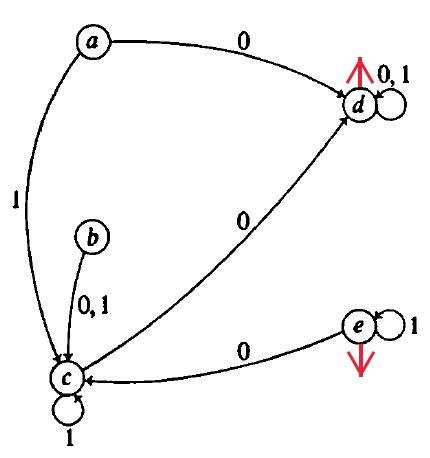
\includegraphics[scale=0.8] {mini-fa} 
	\caption{Finite state automaton}
	\label{fig:mini-fa}
\end{figure}
